\section{CAPÍTULO 4: METODOLOGÍA}\label{cap:methodology}

En este capítulo, se comenzará por discutir el diseño de la investigación para más tarde describir la metodología utilizada para cumplir los objetivos planteados en la Sección~\ref{sec:objectives}. 

\subsection{Diseño de Investigación}

Se ha utilizado un enfoque de investigación cuantitativa para examinar la progresión temporal de la bronquiolitis en pacientes pediátricos. De cara a alcanzar los objetivos planteados en la Sección~\ref{sec:objectives} se discutirá como la muestra limita el cumplimiento de algunos de los objetivos y frente a este límite se van a plantear diferentes alternativas. 

Como ya se ha introducido anteriormente se van a realizar $2$ estudios diferentes con distinto enfoque. A continuación se explicarán por qué se ha decidido realizar 2 estudios diferentes y se discutirán como se deben de replantear los objetivos plantados en la Sección~\ref{sec:objectives}.

Al tener 3 momentos de valoración, que son los que se muestran a continuación:

\begin{enumerate}
    \item $0$ horas $\leq$ Tiempo de Monitorización $<$ $8$ horas 
    \item $8$ horas $\leq$ Tiempo de Monitorización $<$ $16$ horas
    \item $16$ horas $\leq$ Tiempo de Monitorización $<$ $24$ horas
\end{enumerate}


Se ha plantado que se realicen valoraciones del paciente monitorizado antes de terminar el intervalo de monitorización. Es decir, que se valore si al final de las $8$, $16$ y $24$ horas: 

\begin{itemize}
    \item ¿El paciente va a necesitar OAF?
    \item ¿El paciente necesitará ser ingresado en la UCIP?
\end{itemize}

Existe un factor limitante a la hora de hacer estos $3$ estudios predictivos.

En primer lugar es el número de pacientes que han ingresado en la UCIP. Si se parte de los pacientes válidos; \texttt{Valid\_patients\_P1}, definidos en la Sección~\ref{sec:seleccion_pacientes}, que son aquellos que muestran un porcentaje de valores faltantes menor del $5\%$ en las primeras $24$ horas de monitorización, se puede ver cómo solo $4$ han sido llevados a la UCIP, por el contrario existe un mayor registro de pacientes que han necesitado soporte respiratorio mediante el uso de la OAF, $14$. Esta distribución de pacientes se muestra en la Figuras~\ref{fig:bar-OAF-UCIP-valid-1} y \ref{fig:bar-OAF-UCIP-valid-2}. 

\begin{figure}[H]
    \centering
    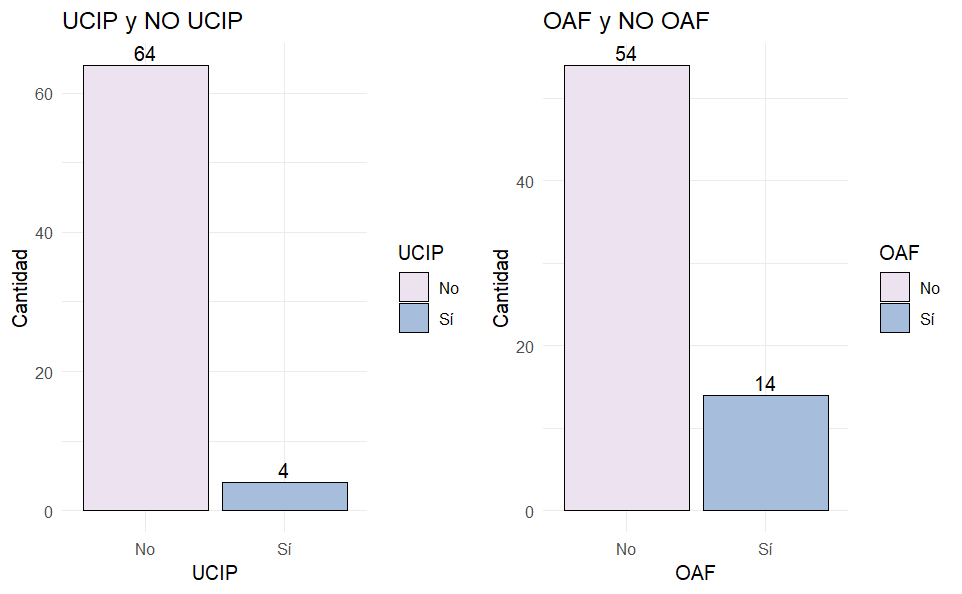
\includegraphics[scale = 0.9]{./img/bar-OAF-UCIP-valid-1.png}
    \caption{Cantidad de pacientes que han sido trasladados a la UCIP y los que NO, que han necesitado OAF y lo que NO, del conjunto de pacientes válidos: \texttt{valid\_patient\_1}}
    \label{fig:bar-OAF-UCIP-valid-1}
\end{figure}

\begin{figure}[H]
    \centering
    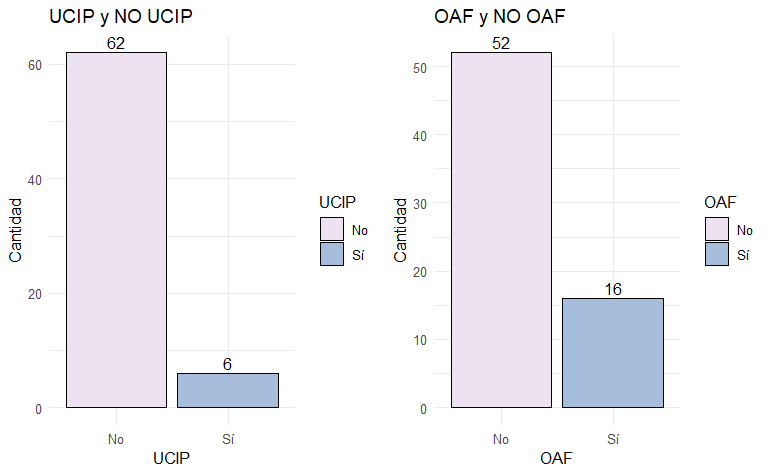
\includegraphics[scale = 0.9]{./img/bar-OAF-UCIP-valid-2.png}
    \caption{Cantidad de pacientes que han sido trasladados a la UCIP y los que NO, que han necesitado OAF y lo que NO, del conjunto de pacientes válidos: \texttt{valid\_patients\_P2}}
    \label{fig:bar-OAF-UCIP-valid-2}
\end{figure}


De cara a plantear la investigación teniendo en cuenta los diferentes intervalos antes mencionados, es necesario ver la distribución de los pacientes dentro de los mismos. Esto se puede ver a continuación en las Figuras \ref{fig:intervalos-valid-1} y \ref{fig:intervalos-valid-2}.

\begin{figure}[H]
    \centering
    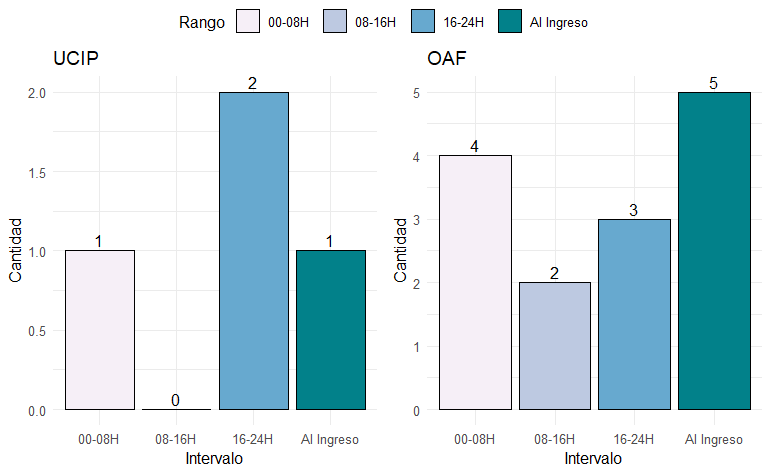
\includegraphics[scale = 0.9]{./img/intervalos-valid-1.png}
    \caption{Distribución de los pacientes dentro de los $3$ intervalos de estudio del conjunto de pacientes: \texttt{valid\_patients\_P1}}
    \label{fig:intervalos-valid-1}
\end{figure}

\begin{figure}[H]
    \centering
    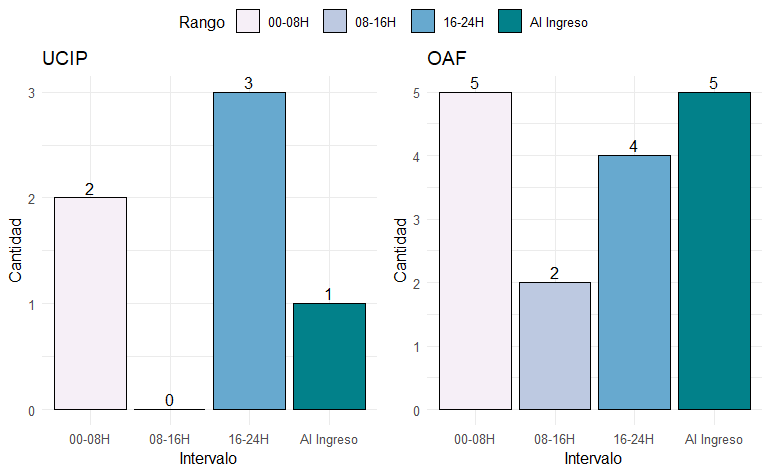
\includegraphics[scale = 0.9]{./img/intervalos-valid-2.png}
    \caption{Distribución de los pacientes dentro de los $3$ intervalos de estudio del conjunto de pacientes: \texttt{valid\_patients\_P2}}
    \label{fig:intervalos-valid-2}
\end{figure}

Una vez vista la distribución de los pacientes que presentan UCIP y OAF en los $3$ intervalos de tiempo antes mencionados, cabe preguntarse si tiene sentido plantear el presente trabajo de la forma previamente discutida.

Respecto a los pacientes que son ingresados en la UCIP, se les va a catalogar como pacientes que han sufrido un DETERIORO. Dado que todos los pacientes que han sido ingresados en la UCIP han recibido soporte respiratorio mediante la técnica OAF, simplemente se les va a considerar como pacientes que han necesitado OAF. En otras palabras, no se utilizará la variable UCIP como variable de salida en este trabajo debido a la escasa representación de este tipo de paciente. Esta consideración se ha mencionado anteriormente en el conjunto total de pacientes en la Figura~\ref{fig:venn-OAF-UCIP} de la Sección~\ref{sec:seleccion_pacientes}.

La exclusión de los pacientes que han necesitado OAF tiene sentido, ya que una vez que al paciente se le suministra OAF, los datos de monitorización recogidos del mismo ya están afectados por la técnica de soporte respiratorio. Por lo tanto, carece de sentido utilizar dichos datos para predecir si el paciente va a necesitar OAF en las próximas $8$ horas, ya que se están recogiendo en un contexto diferente al de los demás pacientes.

Respecto a los pacientes que se les ha aplicado OAF, si excluimos a los pacientes que se les ha aplicado OAF nada más ser ingresados, y aquellos que la han necesitado en las primeras $8$ horas, solo nos quedan 5 pacientes del conjunto de pacientes \texttt{valid\_patients\_P1} y 6 del conjunto de pacientes \texttt{valid\_patients\_P2} que han necesitado OAF para realizar el estudio. La falta de presencia de pacientes de este conjunto se va a abordar mediante la técnica de \textit{oversampling-SMOTE} que se explicará en la Sección~\ref{sec:oversampling}.

Una vez explicado el motivo de la exclusión de los pacientes que han sido ingresados en la UCIP y los que han necesitado OAF, se va a proceder a explicar los $2$ estudios que se van a realizar en la Sección~\ref{sec:estudios}.

\subsubsection{Estudios Realizados}\label{sec:estudios}

\paragraph{Estudio 1}\label{sec:estudio1}

En el \textit{Estudio 1} se considerará al conjunto de pacientes: \texttt{Valid\_patients\_P1}. En este estudio se pretende observar las posibles diferencias entre las \textit{Series Temporales} de monitorización en función de si el paciente ha sido intervenido con OAF o no. Para ello se va a realizar un análisis de la varianza de las medias de las variables de monitorización (\textit{Frecuencia Cardíaca} y \textit{Saturación de O$_2$}) de los pacientes que han necesitado OAF y los que no.

\paragraph{Estudio 2}\label{sec:estudio2}

En el \textit{Estudio 2} se considerará el conjunto de pacientes: \texttt{Valid\_patients\_P2}. En este estudio se pretende observar si es posible predecir si un paciente va a necesitar OAF en las próximas $8$ horas al ingreso. 

Antes de realizar el modelado del algoritmo de clasificación, se va a querer visualizar si mediante el \textit{clustering} de los valores de monitorización de los pacientes se pueden observar diferencias entre los pacientes que han necesitado OAF y los que no. Para la correcta ejecución de lo anteriormente mencionado se seguirán varios pasos:

\begin{enumerate}
    \item \textbf{Selección de Datos:} Al tener 480 valores de monitorización de \textit{Frecuencia Cardíaca} y \textit{Saturación de O$_2$} se van a utilizar diferentes datos para la ejecución de los clusters:
    \begin{enumerate}
        \item \textsc{Datos en bruto:} Se van a utilizar los 480 datos en bruto de monitorización de los pacientes de cada \textit{Serie Temporal}.
        \item \textsc{Función de autocorrelación (FAS):} Se van a utilizar las primeras 50 observaciones de la FAS de cada \textit{Serie Temporal}.
        \item \textsc{Periodograma:} Se usarán los periodogramas de cada \textit{Serie Temporal}.
        \item \textsc{Función de correlación cruzada (FCC):} Se van a utilizar las primeras 100 observaciones de la FCC de la relación entre las \textit{Serie Temporales} de \textit{Frecuencia Cardíaca} y \textit{Saturación de O$_2$}.
    \end{enumerate}
    \item \textbf{Series Temporales a usar:} Se van a utilizar las siguientes transformaciones de los datos seleccionados en el paso anterior:
    \begin{enumerate}
        \item \textsc{Frecuencia Cardíaca y Saturación de O$_2$} Se utilizarán los datos brutos de monitorización de los pacientes.
        \item \textsc{Transformación por Cuantiles de Frecuencia Cardíaca:} Se va a aplicar la transformación por cuantiles a los datos seleccionados en el paso anterior.
        \item \textsc{Frecuencia Cardíaca y Saturación de O$_2$ Escaladas:} Se van a escalar los datos seleccionados en el paso anterior.
    \end{enumerate}
    \item \textbf{Clustering:} Mediante cluster jerárquico se van a agrupar los pacientes en función de los datos seleccionados en el paso anterior.
    \item \textbf{Visualización:} Se van a visualizar los clusters obtenidos en el paso anterior en función de si el paciente ha necesitado OAF de esta forma se pretenderá ver si se aíslan de alguna forma las dos categorías de pacientes previamente establecidas. 
    \item \textbf{Caracterización de Clusters:} 
    Se llevará a cabo la caracterización de los clusters, tomando en consideración las diversas variables descriptivas de cada paciente (edad, género, peso, OAF, ...). Esto se realizará mediante la construcción de un modelo de clasificación discreta, se buscará entender cómo las distintas variables descriptivas influyen en la asignación de etiquetas a los clusters. Este análisis permitirá identificar las variables más influyentes en la distinción de pacientes pertenecientes a los diferentes clusters. Lo ideal en este caso sería observar como en un cluster la variable OAF es la que más influye en la clasificación de los pacientes, ya que esto significaría que los clusters se han formado en función de si el paciente ha necesitado OAF o no. Si esto es así se podría concluir que los clusters obtenidos partiendo de los datos obtenidos de las \textit{Series Temporales} y sus respectivas transformaciones, son capaces de diferenciar a los pacientes que han necesitado OAF de los que no. Respecto a este punto y en último lugar se va a mostrar como se distribuye la importancia de los datos utilizados en función de las etiquetas utilizadas para realizar el \textit{clustering}. En este apartado si los \textit{clusters} generan una muestra de pacientes desbalanceada por grupos se utilizará el método SMOTE para balancearla, esta técnica se explica en la Sección~\ref{sec:oversampling}.
    \item \textbf{Modelado:} Si el anterior paso resulta exitoso será inmediato generar un modelo que permita la clasificación de pacientes que van a necesitar OAF y los que no. El modelo de clasificación será un modelo de clasificación binaria, ya que la variable de salida es una variable categórica con dos categorías: 
    \begin{enumerate}
        \item \texttt{Paciente que Va a Necesitar OAF} 
        \item \texttt{Paciente que NO Va a Necesitar OAF}. 
    \end{enumerate}
\end{enumerate}

Se van a utilizar los datos de las primeras $8$ horas de monitorización de los pacientes, se excluirán aquellos pacientes que ya han sido catalogados como pacientes que han necesitado OAF y se buscará hacer un modelo final para predecir si el paciente después de las 8 primeras horas va a necesitar OAF o no. El Estudio 2 se ha reducido a este planteamiento debido a la limitación de los datos de pacientes que han necesitado OAF, como se ha explicado anteriormente.

\subsubsection{Oversampling}\label{sec:oversampling}

En el campo médico, suele ser común encontrarse con conjuntos de datos donde una categoría tiene significativamente menos observaciones que otra, es decir la proporción de pacientes de cada categoría no está balanceada. Esta disparidad puede afectar negativamente el rendimiento de los modelos de clasificación, ya que pueden tener dificultades para aprender patrones de la clase minoritaria. En el caso de este estudio dónde solo se cuenta con solo 5 pacientes en una categoría (pacientes que ha necesitado OAF posteriormente a las $8$ primeras horas de ingreso) y 40  de la  otra (pacientes que no ha necesitado OAF), existe un claro desequilibrio que puede impactar la precisión de cualquier modelo que se intente construir.

La técnica utilizada en este trabajo, SMOTE (\textit{Synthetic Minority Over-sampling Technique}), es un algoritmo estadístico utilizado para abordar el problema de muestras desbalanceadas en datos de clasificación. En lugar de simplemente duplicar las observaciones de la clase minoritaria, SMOTE crea nuevas muestras artificiales interpolando entre observaciones cercanas. Esto se logra eligiendo una observación de la clase minoritaria y generando puntos artificiales en la dirección de sus vecinos más cercanos de la misma categoría. De esta manera, se aumenta el número de observaciones de la clase minoritaria sin duplicar los mismos puntos (\cite{Chawla2002}).
\newpage

\subsection{Metodología del Estudio 1}\label{sec:metodologia-estudio-1}

En este primer estudio se realizará un análisis de la varianza de las medias de los datos de monitorización de los pacientes pediátricos; los que han necesitado OAF y a los que no la han necesitado. Este análisis de la varianza de los $68$ pacientes pertenecientes del conjunto de datos \texttt{Valid\_patients\_P1} se hará para cada hora de las $24$ totales de monitorización de los pacientes.

Para dicho análisis se hará uso de la prueba $t$ de Student. Esta es una técnica estadística utilizada para comparar las medias de dos grupos (como se presenta en esta situación) y determinar si las diferencias observadas entre ellas son estadísticamente significativas. Se basa en calcular un estadístico $t$ que mide la diferencia entre las medias en términos de la variabilidad dentro de los grupos.

Supongamos que tenemos dos poblaciones, $X$ e $Y$, de las que se han obtenido muestras aleatorias simples con tamaños $n$ y $m$, respectivamente. La hipótesis nula y alternativa se plantean de la siguiente manera:

Hipótesis Nula ($H_0$):
\[
\mu_X = \mu_Y
\]

Hipótesis Alternativa ($H_1$):
\[
\mu_X \neq \mu_Y \quad \text{o} \quad \mu_X < \mu_Y \quad \text{o} \quad \mu_X > \mu_Y
\]

La distribución \( t \) de Student con \( v \) grados de libertad puede definirse como la distribución de la variable aleatoria \( T \) definida por:

\[ T := \frac{Z}{\sqrt{\frac{X}{v}}} \sim t_v \]

donde:

\( Z \sim N(0,1) \) es una variable aleatoria con distribución normal estándar (distribución normal con media 0 y varianza 1).

\( X \sim \chi_{v}^{2} \) es una variable aleatoria que sigue una distribución chi-cuadrada con \( v \) grados de libertad.

\( Z \) y \( X \) son variables aleatorias independientes.

El estadístico \( t \) calculado se compara con un valor crítico de la distribución \( t \) de Student con \( n+m-2 \) grados de libertad para determinar si las diferencias entre las medias son estadísticamente significativas. Si el valor \( p \) asociado con el estadístico \( t \) es menor que el umbral predefinido (nivel de significancia \( \alpha \)), se rechaza la hipótesis nula y se concluye que hay una diferencia significativa entre las medias.


Este estudio se va a realizar para la \textit{Frecuencia Cardiaca}, para la \textit{Frecuencia Cardiaca Transformada por Cuantiles}, para la \textit{Frecuencia Cardiaca Escalada} y para la \textit{Saturación de Oxígeno Escalada}. Se quiere pues observar si realmente existe una diferencia significativa entre las medias de los datos de monitorización de los pacientes pediátricos que han necesitado OAF y los que no la han necesitado.

Para ello partiendo de los $1440$ valores de monitorización se calcularán las medias horarias gracias al código mostrado en la Sección~\ref{sec:anexo2} de los Anexos.




\newpage


\subsection{Metodología Estudio 2}\label{sec:metodologia-estudio-2}

En este segundo estudio como se ha mencionado en la Sección~\ref{sec:estudio2}, se tomará en cuenta el conjunto de pacientes: \texttt{Valid\_patients\_P2}. El propósito de este estudio es investigar la viabilidad de predecir si un paciente requerirá Oxigenoterapia de Alto Flujo (OAF) en las siguientes $8$ horas después del ingreso del paciente.

Para ello habrá que utilizar $2$ herramientas estadísticas que permitan realizar la predicción de la variable de interés:

\begin{itemize}
    \item \textbf{Hierarchical Clustering(HCLUST):} En primer lugar, de manera exploratoria, se agruparán los pacientes en función de las distancias euclídeas entre ellos utilizando el método de clustering \texttt{hclust}. Posteriormente, se evaluará si los grupos generados han aislado en un \textit{cluster} a los pacientes con necesidad de Oxigenoterapia de Alto Flujo (OAF) de aquellos que no la requieren.
    \item textbf{Random Forest Classification (RF):} En segundo lugar, se aplicará el método estadístico \textit{Random Forest} para clasificar a los pacientes según el cluster al que pertenecen, utilizando las variables descriptivas de la Tabla~\ref{tabla:cuali_cuanti}. En este proceso, no se emplearán las variables de \textit{Notas} ni el \textit{Identificador Paciente}. Si se logra aislar a los pacientes que han necesitado OAF, se determinará la importancia directa de la variable \textit{Deterioro}, la cual indica si el paciente ha experimentado OAF o no.
\end{itemize}

\subsubsection{Hierarchical Clustering (HCLUST)}\label{sec:hclust}

Hierarchical Clustering (HCLUST) es una técnica de análisis de datos utilizada para agrupar objetos en función de sus similitudes o distancias. Esta técnica se basa en la construcción de un dendrograma, una estructura jerárquica de ramas que representa la agrupación gradual de los datos (\cite{jain1988algorithms}).

El proceso comienza considerando cada objeto como un grupo individual y luego fusionando iterativamente los grupos más cercanos en función de una medida de similitud o distancia. La distancia puede ser calculada de varias formas, siendo las más comunes y sencilla la distancia euclidiana: 

La fórmula general para calcular la distancia euclídea entre dos objetos \(x_p \) y \(x_q\) es:

\[
d_{euc}(p,q) = \sqrt{(x_p - x_q)^2 + (y_p - y_q)^2}
\]

Esta ecuación puede generalizarse para un espacio euclídeo n-dimensional donde cada punto está definido por un vector de n coordenadas: $p = (p_1,p_2,p_3,...,p_n)$

\[
d_{euc}(p,q) = \sqrt{(p_1 - q_1)^2 + (p_2 - q_2)^2 + \ldots + (p_n - q_n)^2} = \sqrt{\sum_{i=1}^{n}(p_i - q_i)^2}
\]

Hay diferentes distancias que se pueden usar e función del propósito de lo que se quiera hacer con los datos. Cada uno de ellos depende del tipo de datos que se esté utilizando. Se mostrará a continuación una pequeña selección de lo que está disponible en \texttt{R}.
\begin{table}[H]
    \centering
    \caption{Opciones de método de distancia}
    \begin{tabular}{|p{3cm}|p{2.5cm}|p{4.5cm}|p{6cm}|}
    \hline
    \textbf{Medida} & \textbf{Método} & \textbf{Mejor utilizado para...} & \textbf{Cálculo} \\
    \hline
    Distancia euclidiana & euclidean & Datos continuos & \(edist(x, y) = \sqrt{((x_1 - y_1)^2 + (x_2 - y_2)^2 + \ldots)}\) \\
    \hline
    Distancia de Hamming & hamming & Datos categóricos & \(hdist(x, y) = \sum((x_1 \neq y_1) + (x_2 \neq y_2) + \ldots)\) \\
    \hline
    Distancia de Manhattan & manhattan & Diferencias absolutas entre componentes correspondientes & \(mdist(x, y) = \sum(|x_1 - y_1| + |x_2 - y_2| + \ldots)\) \\
    \hline
    Distancia de Canberra & canberra & Valores no negativos (ej. conteos) & \(cdist(x, y) = \sum\left(\frac{|x - y|}{|x + y|}\right)\) \\
    \hline
    Distancia binaria asimétrica de Jaccard & binary & Datos binarios & \(j.dist(x, y) = b + c + d\) (Usando tabla siguiente) \\
    \hline
    \end{tabular}
\end{table}

Una vez que se haya creado una matriz de distancias, es necesario decirle al modelo \textit{HCLUST} que debe entender él como similitud. Esto lleva al próximo punto de decisión: seleccionar qué se entender por \textit{similitud} entre pacientes.

Existen muchas opciones para calcular similitudes entre observaciones. Los métodos \textit{ward.D} y \textit{ward.D2} son generalmente populares y efectivos. Sin embargo, aquí se mostrarán algunas otras opciones diferentes. A continuación se muestra una lista de los métodos de similitud más comunes:

\begin{table}[H]
    \centering
    \begin{tabular}{|p{3.5cm}|p{6cm}|p{6cm}|}
    \hline
    \textbf{Método} & \textbf{Proceso} & \textbf{Resultado} \\
    \hline
    Single & Mide la distancia entre los dos puntos más cercanos en cada cluster & Generalmente es mejor para identificar valores atípicos que no se agrupan bien \\
    \hline
    Complete & Mide la distancia entre los dos puntos más distantes en cada cluster & Generalmente produce clusters más compactos \\
    \hline
    Centroid & Mide la distancia entre el centro de cada cluster & Generalmente funciona mejor para datos con menos similitudes \\
    \hline
    Mediana & Mide la distancia mediana entre el punto mediano de cada cluster & Similar al centroide, pero ponderado hacia donde se encuentran la mayoría de las observaciones \\
    \hline
    Promedio & Mide la distancia promedio entre cada observación en cada cluster, ponderado por el número de observaciones en cada cluster & Generalmente similar a enlace completo, mejor para incorporar valores atípicos \\
    \hline
    Mcquitty & Similar al promedio, pero no toma en cuenta el número de puntos en el cluster & Generalmente similar a enlace simple \\
    \hline
    Ward.D & Minimiza la varianza dentro de los clusters (suma de errores). Combina clusters según la menor distancia entre clusters & Generalmente produce clusters más compactos \\
    \hline
    Ward.D2 & Igual que Ward.D, pero las diferencias están al cuadrado (suma de errores al cuadrado) & Enfatiza las diferencias identificadas en Ward.D, haciendo que los clusters sean más diferenciables \\
    \hline
    \end{tabular}
    \caption{Métodos de enlace y sus resultados}
\end{table}

Una vez establecido que se entiende como similitud el resultado final se muestra en forma de deprograma dónde los pacientes se agrupan gradualmente. Se puede seleccionar el número de grupos al cortar el dendrograma en diferentes alturas. Hay algoritmos que son capaces de calcular el número de grupos más óptimo a considerar como \textit{silouhette} (Sección~\ref{sec:silhouette}) o \textit{gap statistic} que al final son puntuaciones que varían en función del número de \textit{clusters} que se haya decidido previamente.

\textit{HCLUST} tiene la ventaja de ser visualmente intuitivo y permite explorar la estructura de los datos a diferentes niveles de detalle. Sin embargo, su complejidad computacional puede ser alta en conjuntos de datos grandes.

En el contexto de este estudio, se utilizará el método de clustering \textit{HCLUST} para agrupar a los pacientes según sus distancias euclídeas considerando como similitud entre pacientes el método \textit{Ward.D2}. Esto permitirá investigar si los grupos generados pueden destacar diferencias entre pacientes que requieren Oxigenoterapia de Alto Flujo (OAF) y aquellos que no la necesitan.

\paragraph{Silhouette}\label{sec:silhouette}

El método de \textit{Silhouette} es una técnica utilizada para determinar el número óptimo de clusters en un análisis cluster. Proporciona una medida de cómo de similar es un objeto a su propio cluster (cohesión) en comparación con otros clusters (separación). La puntuación de \textit{Silhouette} varía entre -1 y 1, donde una puntuación más alta indica que el objeto está bien ajustado a su propio cluster y mal ajustado a clusters vecinos (\cite{rousseeuw1987silhouettes}).

La fórmula para calcular la puntuación de \textit{Silhouette} \(s(i)\) para un objeto \(i\) se define como:

\[ s(i) = \frac{b(i) - a(i)}{\max\{a(i), b(i)\}} \]

Donde:
\begin{itemize}
    \item \(a(i)\) es la distancia promedio entre el objeto \(i\) y todos los demás objetos en el mismo cluster (cohesión).
    \item \(b(i)\) es la distancia promedio entre el objeto \(i\) y todos los objetos en el cluster más cercano al que \(i\) no pertenece (separación).
\end{itemize}

La puntuación de \textit{Silhouette} para un conjunto de datos se puede calcular promediando las puntuaciones de silueta de todos los objetos:

\[ \text{Puntuación de Silhouette Media} = \frac{1}{N} \sum_{i=1}^{N} s(i) \]

Donde \(N\) es el número total de objetos en el conjunto de datos.

El número óptimo de clusters se elige cuando la puntuación de \textit{Silhouette} media es máxima. Se busca el número de clusters que produce una mayor cohesión dentro de los clusters y una mayor
separación entre los clusters vecinos, lo que refleja en una puntuación \textit{Silhouette} más alta.


\subsubsection{Random Forest (RF)}\label{sec:rf}

Los Random Forest, también conocidos como bosques aleatorios, consisten en un conjunto de árboles de clasificación. Estos bosques se crean mediante un algoritmo que introduce variabilidad en los datos y las variables utilizadas, con el objetivo de reducir la correlación entre los árboles.

El objetivo de los Random Forest es predecir una variable respuesta \(y_i\) en función de \(p\) variables explicativas \(x_i = (x_{1i}, x_{2i}, \ldots, x_{pi})^T\), donde \(N\) es el número total de observaciones en el conjunto de datos. El conjunto utilizado para la estimación se llama \(d = (X, y)\)(\cite{ho1995random}).


\paragraph{CART: Árboles de Clasificación y Regresión}
Los árboles de clasificación (CART) son la base de los algoritmos Random Forest. Estos dividen o segmentan el espacio de los predictores en un número limitado de regiones. Este enfoque pertenece al aprendizaje supervisado, donde se tiene una variable objetivo y se busca establecer una función clasificadora para predecir su valor. CART (Classification and Regression Trees) es una técnica que permite construir árboles de clasificación y de regresión. Se utiliza clasificación cuando la variable objetivo es discreta y regresión cuando es continua.

Dado un conjunto inicial de datos, un árbol de clasificación se construye creando una serie de particiones binarias. Cada partición se llama nodo y divide el espacio en dos partes según una variable. El objetivo es imponer restricciones a los datos a medida que descienden niveles en el árbol para clasificarlos en diferentes conjuntos (\cite{wu2008top}).

Para desarrollar un árbol, es necesario definir dos aspectos:
\begin{itemize}
	\item Cómo se selecciona el criterio de partición de un nodo.
	\item Criterios de parada que determinan cuándo finaliza el proceso de subdivisión.
\end{itemize}


\subparagraph{Criterio de Partición}
Supongamos que tenemos \(p\) variables explicativas o predictores: \(x_1, x_2, \ldots, x_p\). Tomemos la primera variable \(x_1\) y busquemos el valor \(s\) que divide la muestra en dos regiones que cumplan:

\[
R1 = \{x_{1i} \mid x_{1i} < s\} \quad \text{y} \quad R2 = \{x_{1i} \mid x_{1i} \geq s\}
\]

Es decir, o se toma una de las variables explicativas (o predictores) de tus datos y se busca un valor $s$ que divida las observaciones en dos grupos: uno donde los valores de esa variable son menores que $s$ y otro donde son mayores o iguales a $s$.

Y que minimice:

\[
RSS_1(s) = \sum_{i \in R_1} (y_i - \bar{y}_{R_1})^2 + \sum_{i \in R_2} (y_i - \bar{y}_{R_2})^2
\]
Donde \(\bar{y}_{R_1}\) y \(\bar{y}_{R_2}\) son las medias de la variable \(y\) en las regiones \(R_1\) y \(R_2\). Esto se hace pues se pretende que en cada grupo la variable respuesta \(y\) sea lo más homogénea posible. Se busca la variable $s$ que minimice la suma de los cuadrados de las diferencias entre los valores de $y$ y la media de $y$ en cada grupo.

Elegido \(s\) óptimo para \(x_1\), se repite el proceso con \(x_1, x_2, \ldots, x_p\). De las \(p\) variables, se elige para la partición la que resulte en la menor \(RSS_j\).

El proceso se repite, pero ahora se tratan de manera independiente los conjuntos \(R_1\) y \(R_2\). El proceso continúa hasta que se alcance el criterio preestablecido de parada y se definan los nodos terminales \(R_1^*, R_2^*, \ldots, R_j^*\). El objetivo es lograr una partición de estos nodos que minimice:

\[
RSS_T = \sum_{j=1}^{J} \sum_{i \in R_j^*} (y_i - \bar{y}_{R_j^*})^2
\]

\subparagraph{Criterio de Parada}
Existen varios criterios de parada para limitar el crecimiento del árbol:
\begin{itemize}
	\item Parámetro de Complejidad: Este parámetro se refiere al aumento en el valor de \(R^2\) al agregar una rama al árbol. Se establece un umbral para el cual agregar más ramas al árbol no aumenta significativamente el valor de \(R^2\).
	\item Minsplit: Se detiene el crecimiento del árbol cuando el número de observaciones en un nodo es menor que un umbral predefinido.
	\item Maxdepth: Se detiene el crecimiento cuando la profundidad de las ramas del árbol supera un umbral establecido.
\end{itemize}
La recomendación general es encontrar el árbol más pequeño que maximice el valor de \(R^2\).

\subparagraph{Ventajas de los CART}
Los árboles CART presentan varias ventajas:
\begin{itemize}
	\item No se requiere preparación de los datos de entrada.
	\item Pueden manejar variables faltantes.
	\item Son efectivos para grandes bases de datos con diversas variables.
	\item Son fáciles de entender e interpretar.
\end{itemize}

\subsubsection{Algoritmo de creación del Random Forest}

Para \(b = 1,2, \ldots, B\), se realiza lo siguiente:
- Se elige una muestra de tamaño \(N\) de manera aleatoria y con reemplazo del conjunto de datos total. Esto se llama bootstrap.
- Se construye un árbol llamado \(r_b(x)\), y en cada nodo del árbol se utilizan \(m \ll p\) variables de las \(p\) variables del conjunto de datos. La elección común para \(m\) es \(m = \sqrt{p}\).
- El conjunto de árboles formados, \(r_b(x)\) para \(b = 1,2, \ldots, B\), se llama Random Forest.

\paragraph{División del conjunto de datos}

En general, los algoritmos de Machine Learning dividen el conjunto de datos en dos partes: una para estimación o entrenamiento, y la otra para test o validación.

\paragraph{DEstimación del error en la predicción de variables de respuestas continuas}

La predicción para \(x_i = (x_{1i}, x_{2i}, \ldots, x_{pi})^T\) se calcula como:

\[ \hat{y}_i = \hat{r}_{rf}(x_i) = \frac{1}{B} \sum_{b=1}^{B} \hat{r}_b(x_i) \]

Donde \(B\) es el número de árboles en el Random Forest.

El error se define como:

\[ e_i = y_i - \hat{y}_i \]

El error cuadrático medio (MSE) se calcula como:

\[ MSE = \frac{1}{n} \sum_{i=1}^{n} e_i^2 \]

El coeficiente \(R^2\) se define como:

\[ R^2 = 1 - \frac{\sum_{i=1}^{n} e_i^2}{\sum_{i=1}^{n} (y_i - \bar{y})^2} \]

La desviación típica residual \(S_{\hat{R}}\), siendo \(m\) el número de observaciones en el conjunto de validación, se calcula como:

\[ S_{\hat{R}} = \sqrt{\frac{e_i^2}{m-1}} \]

\paragraph{OOB error (Error fuera de la bolsa)}\label{sec:oob}

El OOB error es una medida de error aplicada a modelos que utilizan la técnica de boostrapping. Dado que aproximadamente \(1/3\) de los datos nunca se seleccionan debido al reemplazo, el OOB representa el error de predicción cometido por el Random Forest en los valores que quedaron fuera de la muestra.

\paragraph{Importancia de las variables}\label{sec:importancia-variables}

Un modelo Random Forest funciona como una caja negra y proporciona buenas predicciones. Sin embargo, no brinda información sobre cada variable explicativa.

La importancia de una variable se puede calcular en función de cómo afecta a la salida del modelo cuando se realizan cambios en las variables de entrada. A continuación, se describen dos formas de calcular la importancia.

\subparagraph{Índice de la pureza de los nodos}

En el contexto de Random Forest, el Índice de la Pureza de los Nodos se refiere al proceso de evaluación de la contribución de cada variable al proceso de particionamiento de los datos en los nodos de cada árbol. Al utilizar una variable en un nodo, se cuantifica la reducción de la variabilidad explicada por la partición resultante. Estos valores de reducción se acumulan para todas las variables y árboles, generando una medida conocida como la importancia de la variable. Las variables que exhiben una mayor capacidad para reducir la variabilidad en los nodos se consideran más importantes en el proceso de toma de decisiones del Random Forest.

\subparagraph{Incremento del Mean Squared Error  \texttt{\%IncMSE}}

El índice \texttt{\%IncMSE} en el contexto de Random Forest mide el incremento en el Error Cuadrático Medio (MSE) a través de la realización de una permutación aleatoria en una de las variables de entrada. La disparidad entre el MSE antes y después de la permutación se normaliza y se promedia para determinar la relevancia de la variable en el proceso de modelado. Este índice proporciona una evaluación cuantitativa de cómo la perturbación de una variable afecta la precisión de las predicciones, identificando así las variables que tienen un mayor impacto en los resultados del Random Forest. Una variable que su permutación genere una gran variación será considerada como importante. Por el contrario, una variable que no afecte la precisión de las predicciones será considerada como no importante.

En resumen, los Random Forest son una poderosa técnica de aprendizaje automático que combina múltiples árboles de clasificación para realizar predicciones más precisas y robustas. Su proceso de creación introduce variabilidad y utiliza técnicas como el OOB error y la importancia de variables para mejorar su rendimiento y capacidad de generalización.

\newpage